\documentclass[MASTER.tex]{subfiles} 
\begin{document} 

%=================================================%
\begin{frame}
\frametitle{Main features of ggplot2}
\Large
\begin{itemize}
	\item Create graphics using \texttt{qplot} or \texttt{ggplot}
	\item Add layers to an existing plot using ``\texttt{+}"
	\item Change aesthetics by variables in the data
	\item Control the type of plot using \texttt{geom}s
	\item Panel by variables using the \texttt{facet\_$\ast$} functions
\end{itemize}

\end{frame}
%=================================================%
\begin{frame}[fragile]

		\frametitle{Tube Data with ggplot2}
		\Large
	\begin{framed}
		\begin{verbatim}
		library(ggplot2)
		qplot(Month, Excess, data = tubeData) +
			   geom_smooth(method = "lm", 
					     col = "red") +
			  facet_wrap(~Line) +
			  theme_bw()
		
		\end{verbatim}
	\end{framed}
\end{frame}
%=================================================%
\begin{frame}[fragile]
	\frametitle{The \texttt{geoms}}
\Large
ggplot2 includes a variety of \texttt{geom}s for
		controlling the type of plot we create

\begin{figure}
\centering
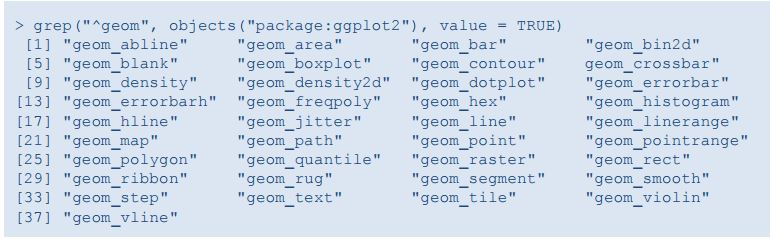
\includegraphics[width=1.05\linewidth]{gott-geoms}
\end{figure}


\end{frame}
%=================================================%
\begin{frame}
	\Large
	\frametitle{Facetting}
	\begin{itemize}
		\item We can panel graphics based on variables in the
		data using facets
		\item \texttt{facet\_wrap} and \texttt{facet\_grid} add panels as layers
	\end{itemize}
\end{frame}
%=================================================%

%=================================================%
\begin{frame}
	\frametitle{Scales and Themes}
	\Large
	\begin{itemize}
		\item ggplot2 provides a large number of scale functions
		to control aspects of a graphic including axes and
		legends
		\item theme functions allow us to control the overall style
		of the graphic
	\end{itemize}
	
	
\end{frame}
%======================================================== %
\end{document}